\documentclass[10pt]{beamer}
\usepackage[german]{babel}
\usepackage[utf8]{inputenc}
\usepackage{textgreek}
\usepackage{units}

\usepackage[official]{eurosym}


\title[soldering-workshop] % (optional, only for long titles)
{Lötworkshop für Anfänger}
\author{Eileen, Towa, Andi, Klaus}
\usetheme{metropolis}

\begin{document}
    \maketitle
    
    
    \begin{frame}
    \frametitle{Inhalt}
    \begin{itemize}
    	\item{Was bedeutet Löten?}
    	\item{Benötigte Gegenstände}
    	\item{Wie wird gelötet?}
    	\item{Praxisteil: Löten der Maschinendeck Badge}
    \end{itemize}
	\end{frame}
    
    \begin{frame}
    \frametitle{Was ist Löten?}
    \begin{itemize}
    	\item{Verbindung zweier Metalloberflächen mit einer Metalllegierung niedrigerer Schmelztemperatur}
    \end{itemize}
	% Bildquellen: https://qph.fs.quoracdn.net/main-qimg-9fcaa4b47839d57b306a2613972ada02.webp
	% https://www.makerspaces.com/how-to-solder/
	\begin{figure}[hbtp]
		\centering
		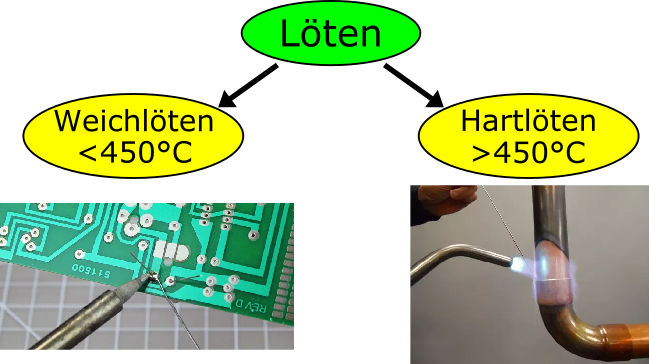
\includegraphics[width=\linewidth*2/3]{images/weich_hartloeten.png}
	\end{figure}
	\end{frame}

	\begin{frame}
	\frametitle{Elektroniklöten}
	\begin{itemize}
		%TODO: Bilder von Elektronischen Bauteilen und einer Platine
		\item{Verbinden von elektronischen Bauteilen mit einer Platine (PCB)}
		\item{Verwendung von Handlötkolben oder Lötstationen mit \unit[300 - 400]{$^\circ$C} und \unit[30 - 100]{W}}
		\item{Als Metallegierung wird Lot oder Lötzinn verwendet}
	\end{itemize}
	\end{frame}

	\begin{frame}
	\frametitle{Das Lot}
	\begin{itemize}
		\item{Metalllegierung aus Zinn, Blei und anderen Metallen (Elektroniklot)}
		\item{Flußmittelseele zur Verbesserung der Flusseigenschaften im Lot enthalten}
		\item{\textcolor{red}{Beim Erhitzen des Lötzinns können Flussmittelspritzer auftreten. Deshalb nicht zu nahe mit dem Gesicht an die Lötstelle gehen!}}
		\item{\textcolor{red}{Blei ist ein giftiges Schwermetall! Nicht verschlucken!}}
	\end{itemize}
	\begin{figure}[hbtp]
		\centering
		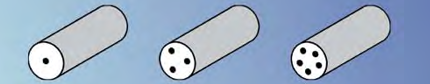
\includegraphics[width=\linewidth]{images/lotseele.png}
		\caption{Quelle: ERSA Lötfibel}
	\end{figure}
	\end{frame}

	\begin{frame}
	\frametitle{Was wird benötigt?}
	\begin{itemize}
		\item{Bausatz}
		\item{Lötkolben}
		\item{Lötzinn}
		\item{Seitenschneider}
		\item{Schwamm / Trockenreiniger}
	\end{itemize}
	\end{frame}

	\begin{frame}
	\frametitle{Optionales Zubehör}
	\begin{itemize}
		\item{Lötstation}
		\item{Pinzetten}
		\item{Dritte Hand}
		\item{Lötdampfabsaugung}
		\item{Lupe}		
		
		\item{Heißluftlötkolben}
		\item{Lötpinzette}
	\end{itemize}
	\end{frame}

	\begin{frame}
	\frametitle{Lötvorgang}
	% evt. vorher noch reinigen
	\begin{columns}[T] % align columns
		\begin{column}{.33\textwidth}
			\textbf{Benetzen} \newline
			Auf die gereinigte Lötspitze etwas Lot geben.
		\end{column}%
		\hfill%
		\begin{column}{.33\textwidth}
			\textbf{Fließen} \newline
			Die Lötstelle erhitzen und soviel Lot dazu geben wie nötig.
		\end{column}%
		\begin{column}{.33\textwidth}
			\textbf{Binden} \newline
			Erst Lot, dann Spitze von Lötstelle entfernen und anschließen abkühlen lassen.
		\end{column}%
		\hfill%
	\end{columns}
	\end{frame}

	\begin{frame}
	\frametitle{Löten 101}
	\begin{figure}[hbtp]
		\centering
		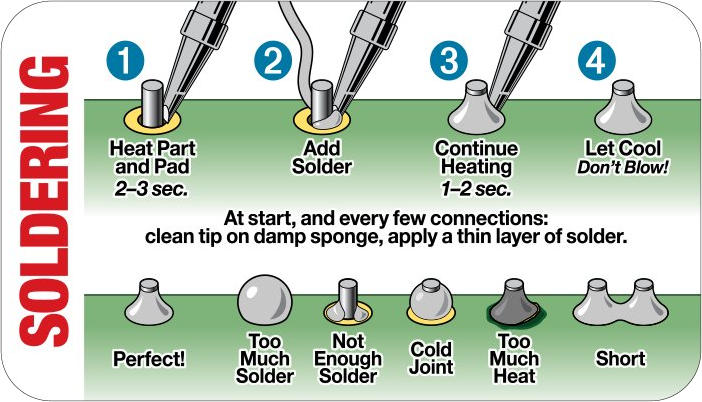
\includegraphics[width=\linewidth]{images/solder.png}
		\caption{Quelle: Adafruit}
	\end{figure}
	\end{frame}

	\begin{frame}
	\frametitle{Praxisteil: Vorbereitung}
	\begin{itemize}
		\item{Arbeitsplatz überprüfen: Lötkolben, Seitenschneider, Lötzinn, Schwamm, Bausatz vorhanden}
		% TODO: Lötkolben vorheizen evt. am Anfang
		\item{Lötkolben/Lötstation vorgeheizt (\unit[350]{$^\circ$C})}
		\item{Bausatz auspacken und Teile überprüfen}
	\end{itemize}
	\begin{figure}[hbtp]
		\centering
		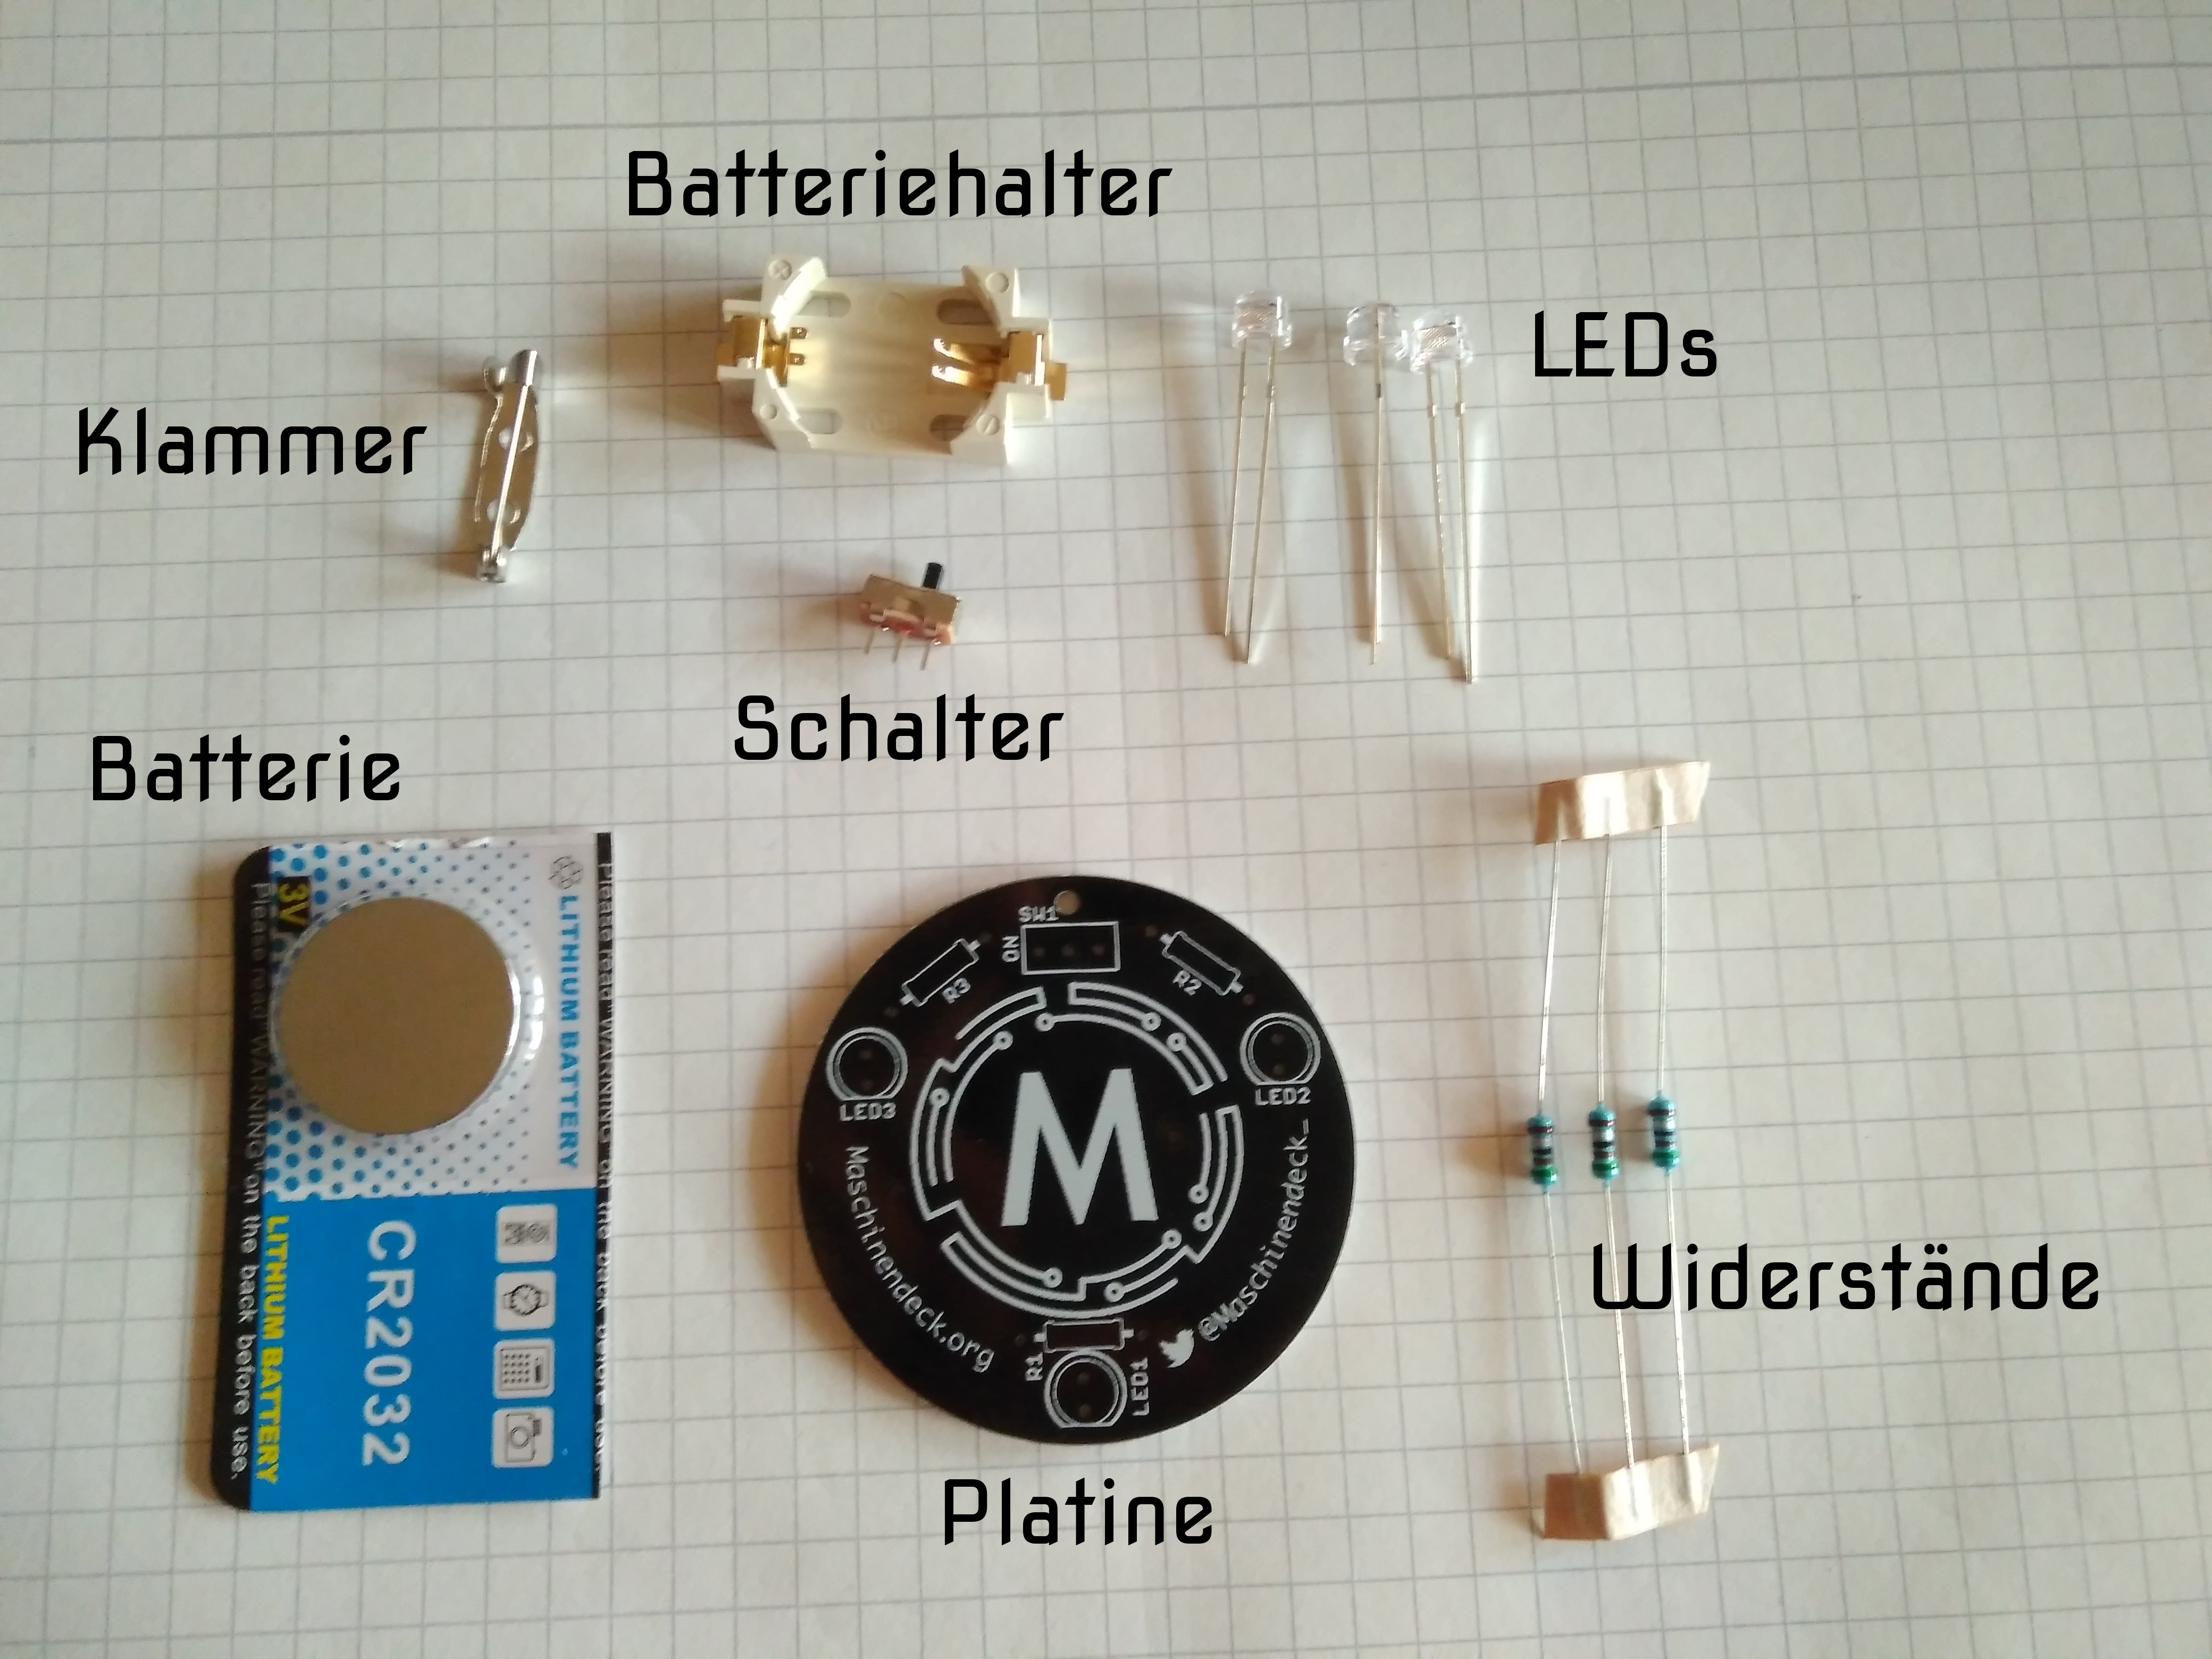
\includegraphics[width=\linewidth*5/10]{images/badge.jpg}
		\caption{Der Bausatz}
	\end{figure}
	\end{frame}

	\begin{frame}
	\frametitle{Schritt 1: Löten der Widerstände}
	Die Widerstände sind recht unempfindlich und sind perfekt geeignet für die ersten Lötstellen
	\begin{enumerate} 
		\item{Widerstände mithilfe der Biegehilfe passend biegen}
		\item{Widerstände durch die entsprechenden Löcher in der Platine stecken}
		\item{Anschlussdrähte auf der anderen Seite der Platine etwas auseinanderbiegen}
		\item{Platine umdrehen und Widerstände festlöten}
	\end{enumerate}
	\end{frame}

	\begin{frame}
		\frametitle{Schritt 1: Löten der Widerstände}
		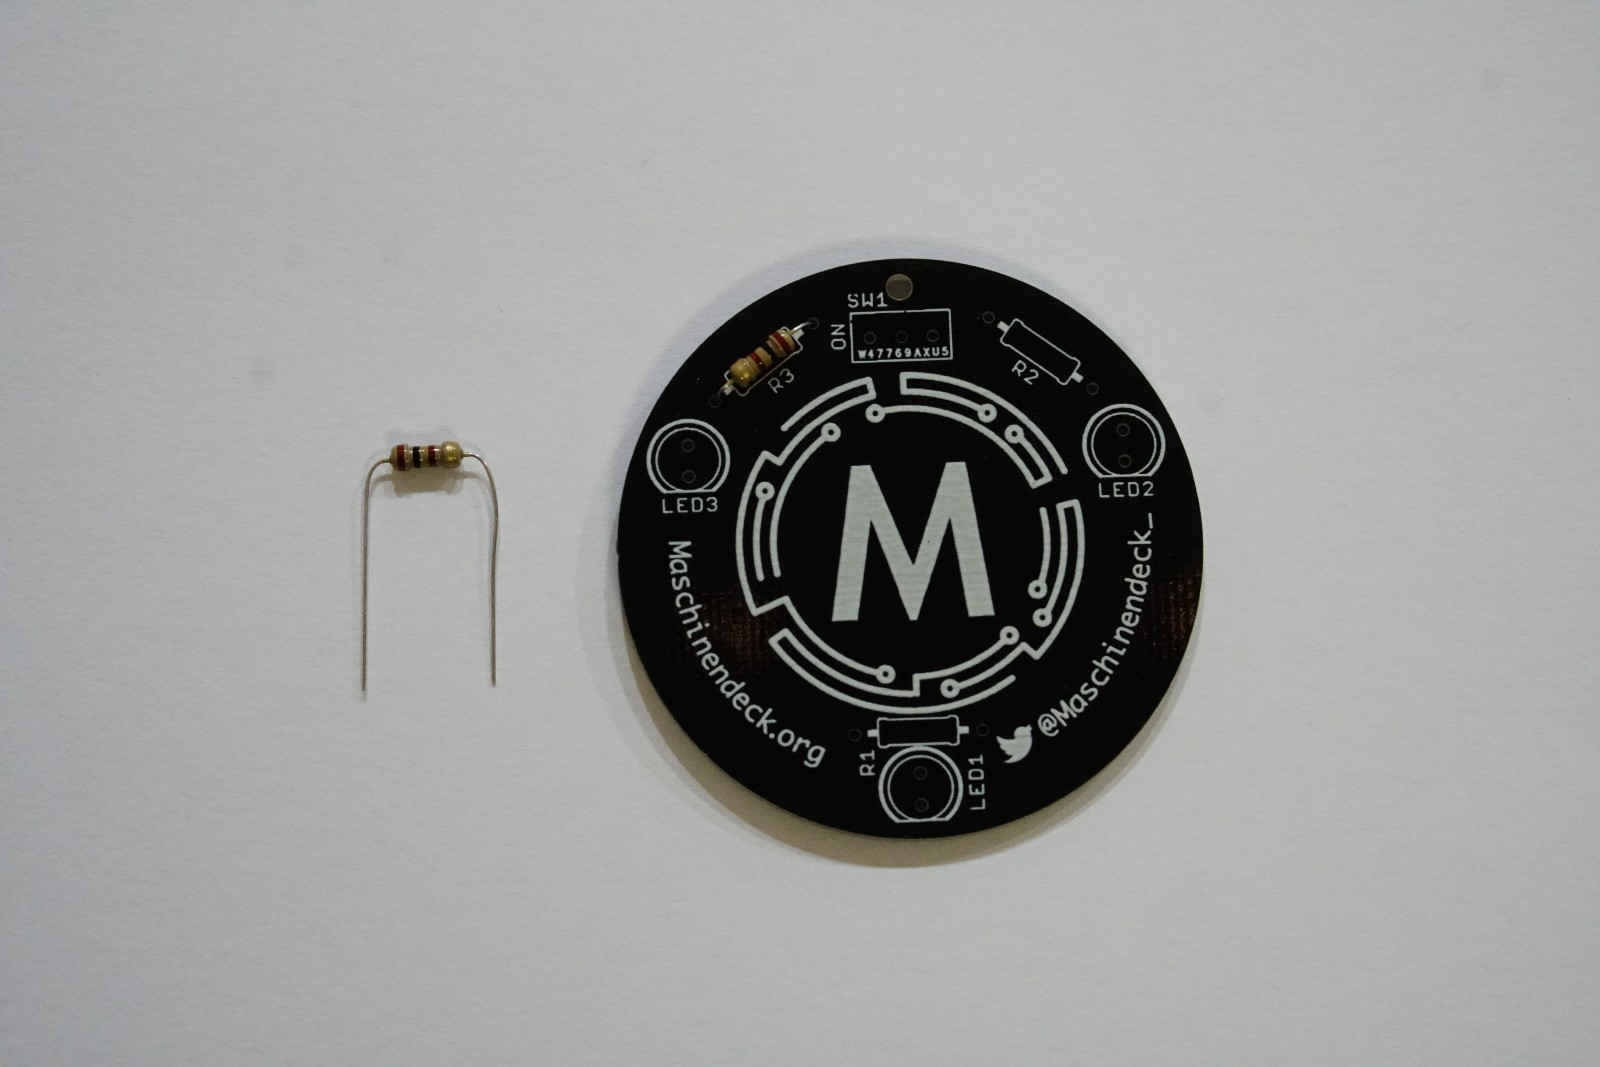
\includegraphics[width=\linewidth]{images/badge18/resistor.JPG}
	\end{frame}
	
	\begin{frame}
	\frametitle{Schritt 2: Löten der LEDs}
	LEDs sind empfindlich gegenüber großer Hitze. Sie sollten nicht unnötig lange erhitzt werden
	\begin{enumerate} 
		\item{LEDs durch die entsprechenden Löcher stecken (darauf achten, dass die abgeflachte Seite der LED mit dem Aufdruck auf der Platine übereinstimmt)}
		\item{Anschlussdrähte etwas auseinander biegen}
		\item{Platine Umdrehen und LEDs festlöten}
	\end{enumerate}
	\end{frame}

	\begin{frame}
		\frametitle{Schritt 2: Löten der LEDs}
		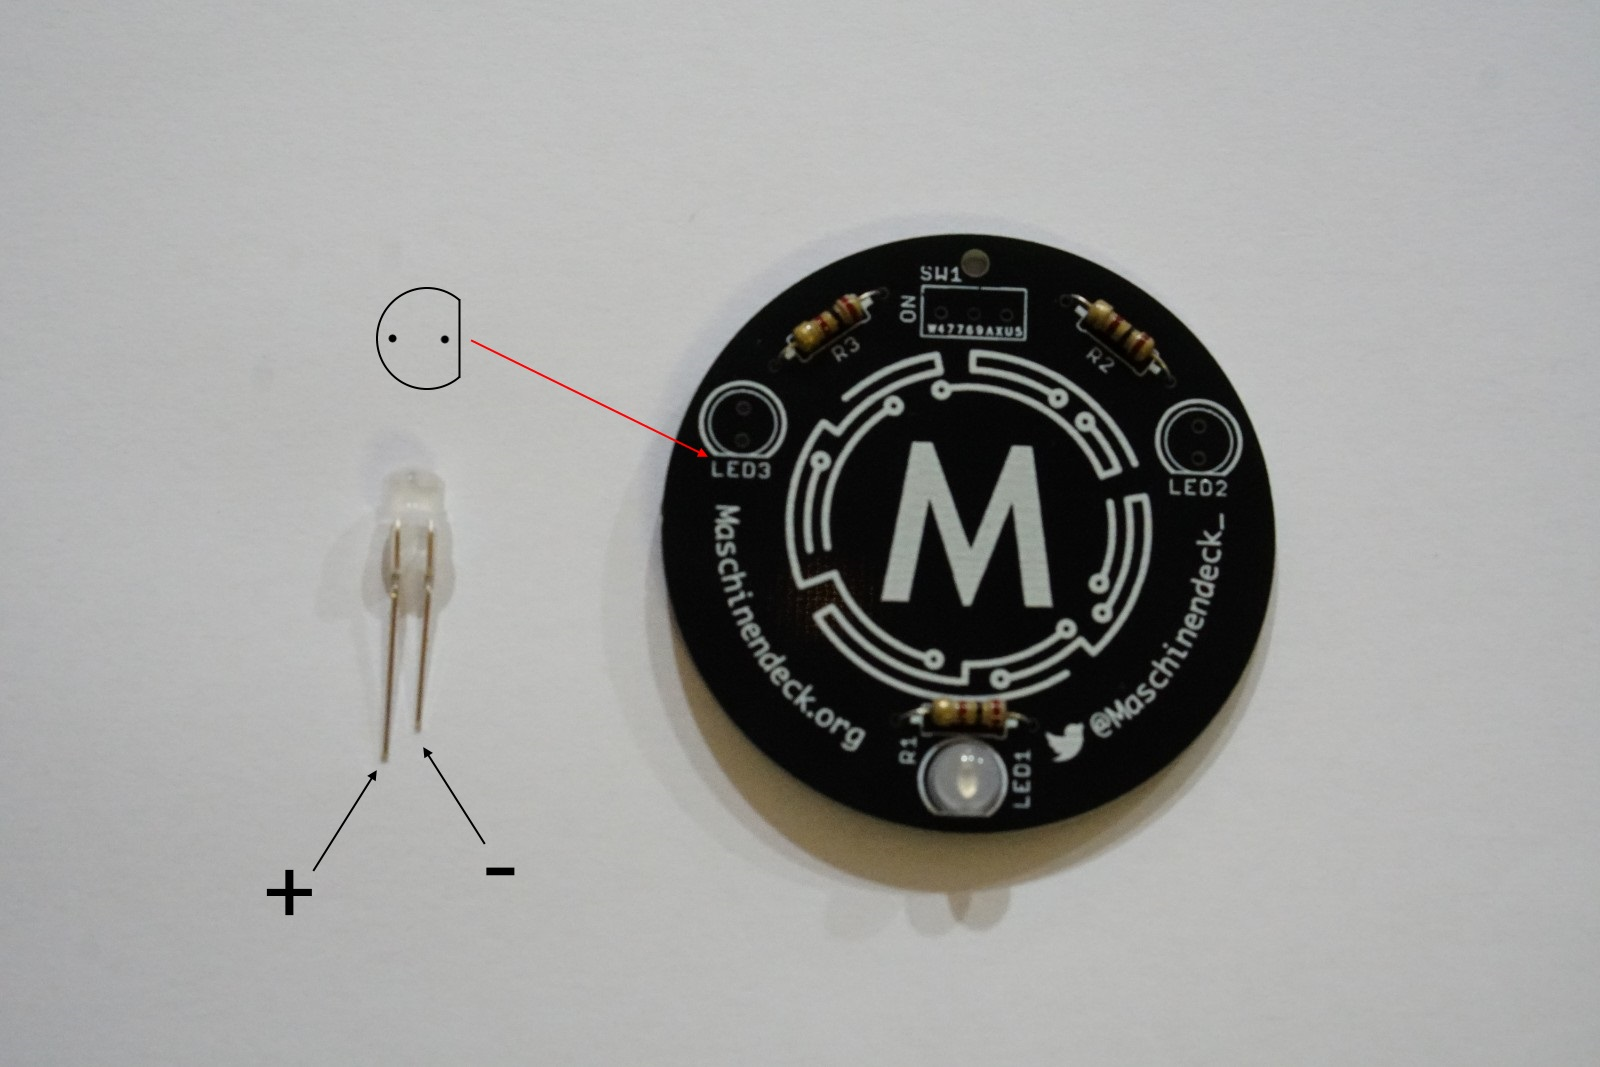
\includegraphics[width=\linewidth]{images/badge18/ledPolarity.JPG}
	\end{frame}

	\begin{frame}
	\frametitle{Schritt 3: Löten des Batteriehalters}
	Der Batteriehalter wird auf der Oberfläche verlötet (SMD).
	\begin{enumerate} 
		\item{Batteriehalter richtig herum auf die Platinenunterseite legen}
		\item{Etwas Lötzinn an die Lötspitze auftragen}
		\item{Batteriehalter mit der Pinzette festhalten und mit der anderen Hand eine Lötstelle festlöten}
		\item{Andere Seite wie gewohnt festlöten}
		\item{Nachdem die andere Seite gelötet ist, kann die erste Seite noch einmal nachgelötet werden}
	\end{enumerate}
	\end{frame}

	\begin{frame}
		\frametitle{Schritt 3: Löten des Batteriehalters}
		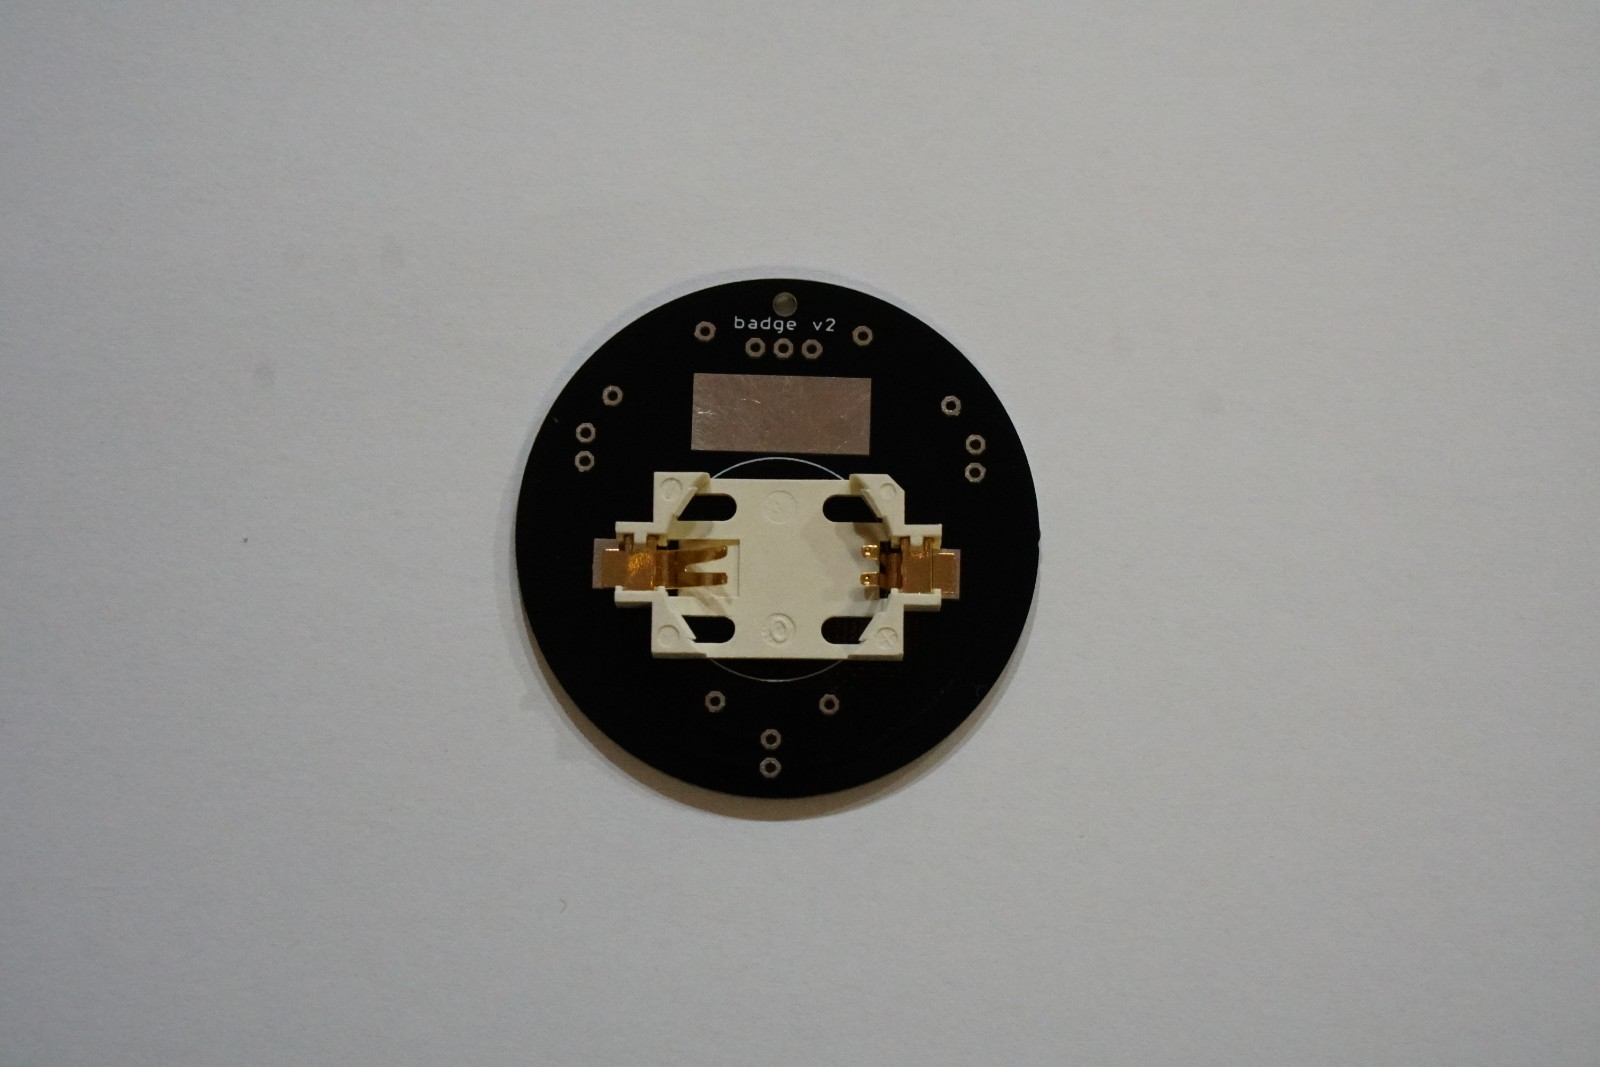
\includegraphics[width=\linewidth]{images/badge18/battHolderInPlace.JPG}
	\end{frame}

	\begin{frame}
	\frametitle{Schritt 4: Löten der Anstecknadel}
	Die Anstecknadel ist sehr groß und muss deshalb länger erhitzt werden.
	\begin{enumerate} 
		\item{Anstecknadel aufmachen und auf das Pad legen}
		\item{Anstecknadel erhitzen und viel Lötzinn auftragen}
		\item{Sobald die Nadel gut benetzt ist, kann diese noch mit der Pinzette richtig ausgerichtet werden}
	\end{enumerate}
	\end{frame}

	\begin{frame}
		\frametitle{Schritt 4: Löten der Anstecknadel}
		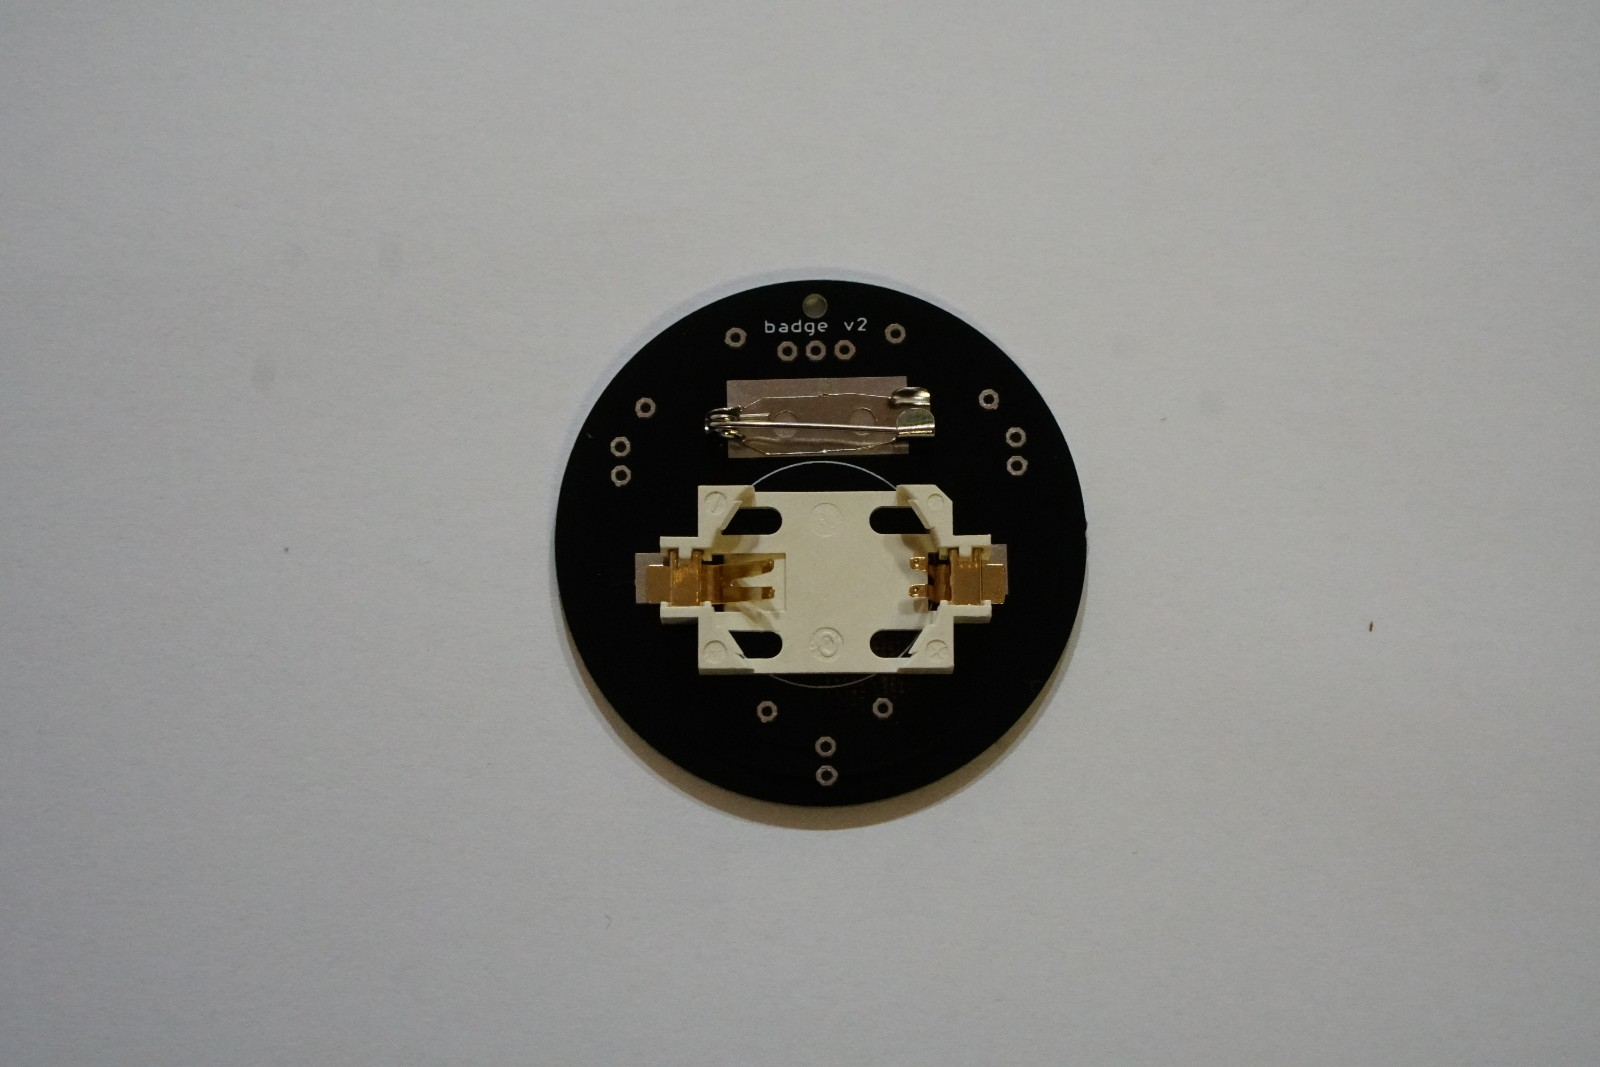
\includegraphics[width=\linewidth]{images/badge18/needleAndHolder.JPG}
	\end{frame}

	\begin{frame}
	\frametitle{Schritt 5: Löten des Schalters}
	\begin{enumerate} 
		\item{Den Schalter von der Vorderseite durch die Platine stecken (Orientierung egal)}
		\item{Platine auf den Schalter legen und diesen auf der Unterseite an einer Lötstelle verlöten}
		\item{Falls der Schalter schief sitzt, kann er vorsichtig auf der Vorderseite gerade gedrückt werden während man die Lötstelle erneut erhitzt (Vorsicht: Verbrennungsgefahr)}
		\item{Zum Schluss die restlichen Lötstellen verlöten}
	\end{enumerate}
	\end{frame}

	\begin{frame}
		\frametitle{Schritt 5: Löten des Schalters}
		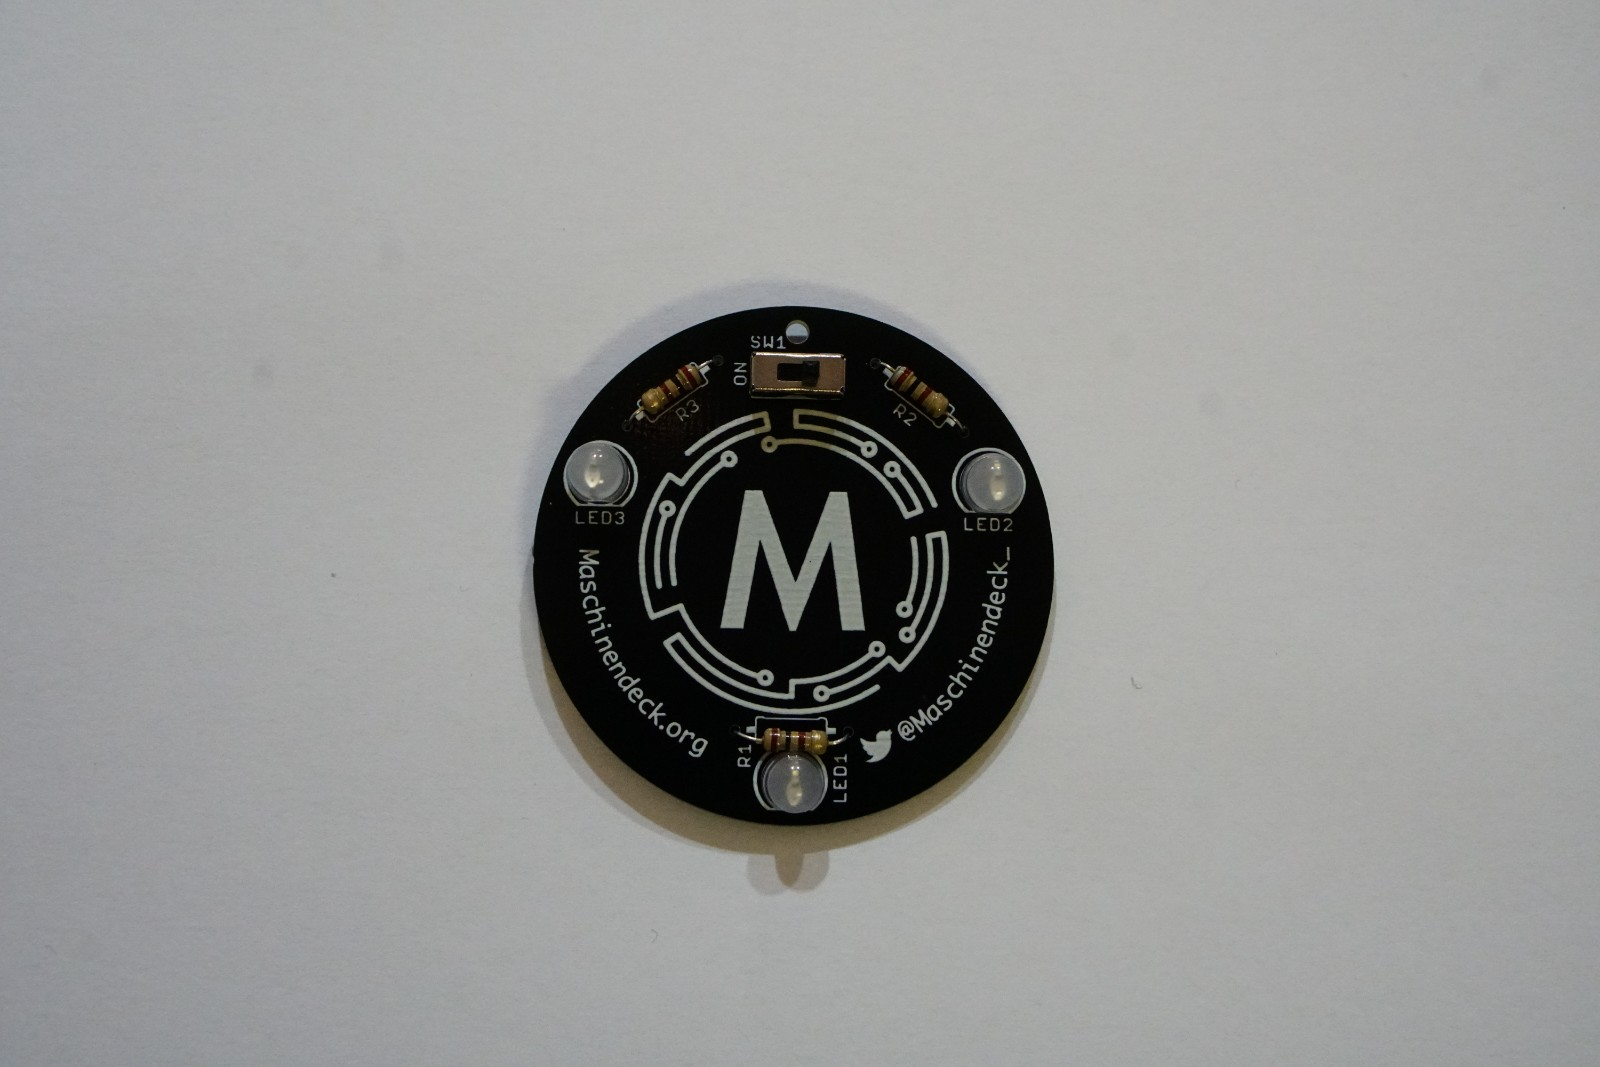
\includegraphics[width=\linewidth]{images/badge18/final.JPG}
	\end{frame}

	\begin{frame}
	\frametitle{Zum Schluss}
	\begin{itemize} 
		\item{Batterie einlegen und den Schalter auf ``ON'' stellen}
		\item{Lötstationen ausschalten}
		\item{Lötspitze nicht reinigen, da das verbleibende Lötzinn auf der Spitze eine Schutzschicht bildet}
		\item{Die Platine kann optional noch mit Alkohol oder Isopropanol gereinigt werden}
	\end{itemize}
	\end{frame}

	\begin{frame}
		\frametitle{Zum Schluss}
		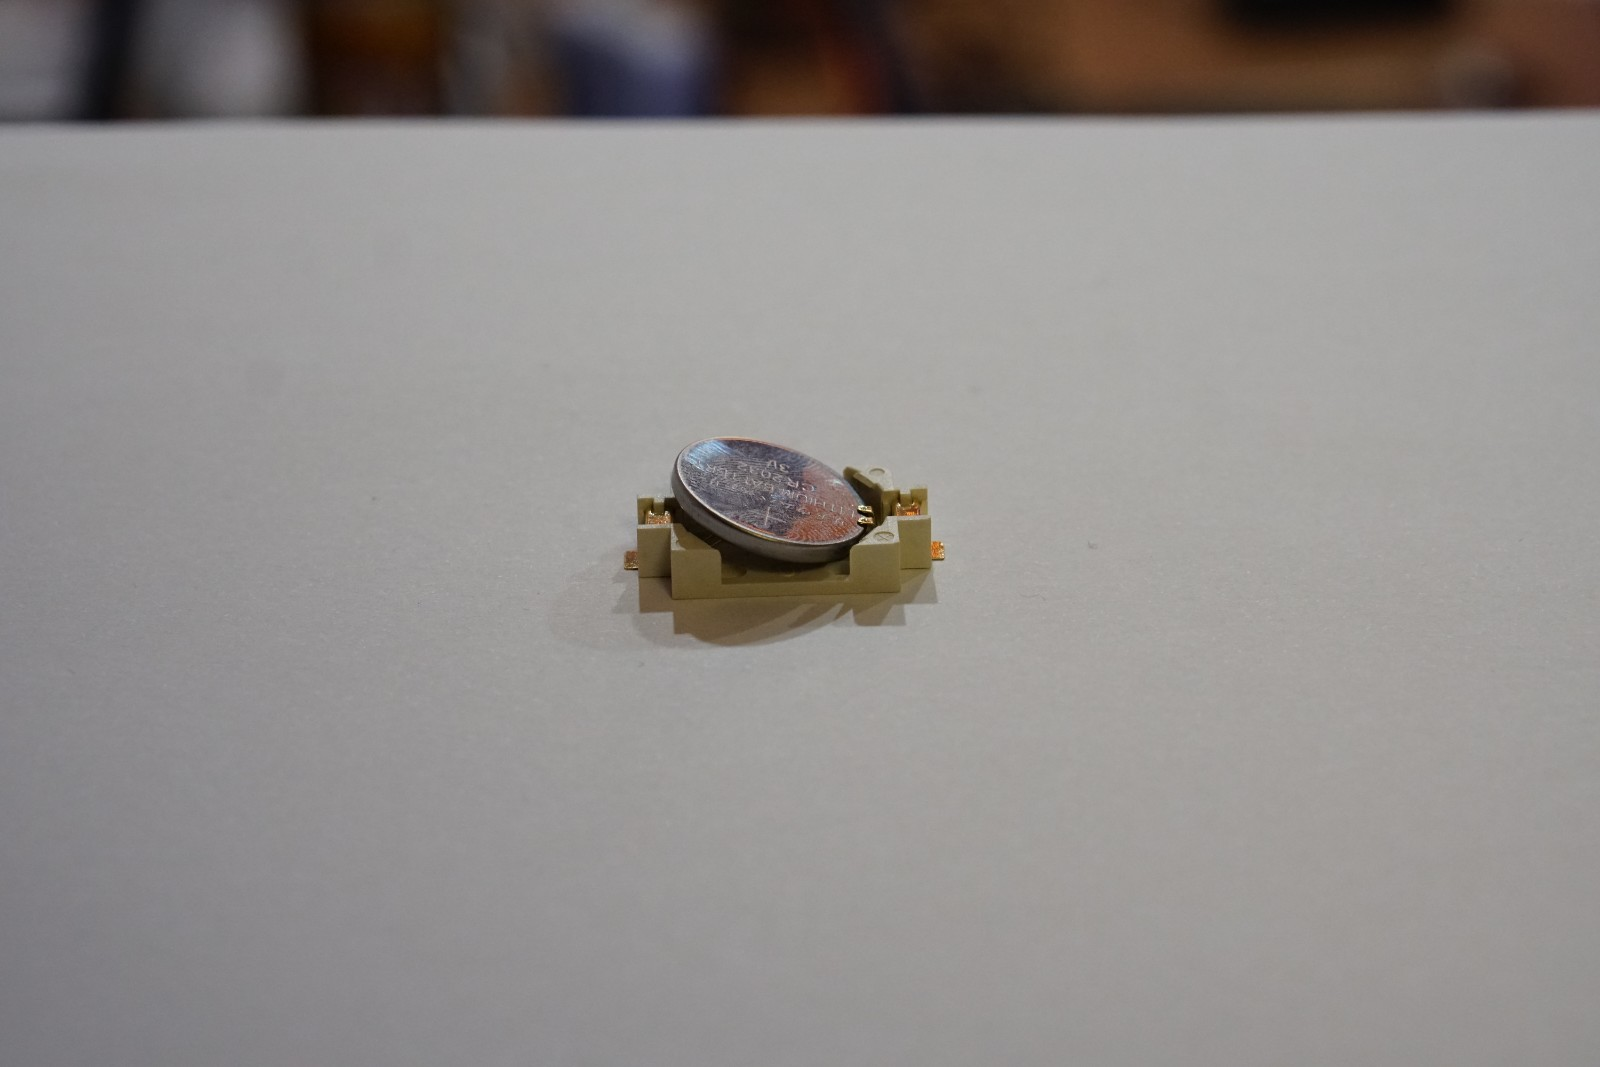
\includegraphics[width=\linewidth]{images/badge18/battHolderWithBattery.JPG}
	\end{frame}

	\begin{frame}
		\frametitle{Quellen für Lötzubehör und Bausätze}
		Ein einfacher Lötkolben kostet unter 10\euro{}, brauchbare Stationen sind bereits für 40\euro{} zu haben!
		
		\begin{itemize}
			\item{ELV (www.elv.de)}
			\item{Watteroth (www.watterott.com)}
			\item{Reichelt (www.reichelt.de)}
		\end{itemize}
	\end{frame}

	\begin{frame}
	\frametitle{Vielen Dank}
	\centering
	{\LARGE Vielen Dank für Ihre Aufmerksamkeit!}
	\end{frame}
    
\end{document}
